\section{Problemanalyse}
For at besvare det initierende problem, er det nødvendigt at researche. Heraf opstilles der en række hv-spørgsmål, som vil danne grundlag for problemfeltet. Formålet med disse spørgsmål er, at komme i dybden med samt at forstå problemet.
\clearpage
\subsection{Relevans}
\subsubsection{Lyset påvirkning på mennesket}

Undersøgelser har vist at lys har stor invirkning på vores humør og trivsel.
Blåt/hvidt lys har den effekt at vi føler os mere vågne og oppe på mærkerne\cite{videnskab_dk_paavirkning}, hvorimod rødt/gult lys har den modsatte effekt. Vi bliver mere afslappede og dermed trætte. Det giver god mening når vi ser på det lys solen udsender om dagen(hivdt/blå himmel), som gør os friske, og det lys vi ser når solen går ned(rød solnedgang/bål om natten) og det er tid til at gå til ro. Vi bruger også lys til rigtig meget i hverdagen. Øjet, som virker ved hjælp af lys bruger vi til at navigere, se evt. farer og genkende venner. Når vi bruger en computer er vi afhængige af at kunne se skærmen for at kunne bruge den. Mange mennesker sidder i kontormiljøer i stort set al deres arbejdstid og er afhængige af at lyset er godt. Hvis lyset ikke er godt vil man ofte blive træt og uproduktiv. Derfor er det vigtigt at både loftlamper, skrivebordslamper og indretningen spiller godt sammen og skaber et godt lys-miljø.


\subsubsection{Når lampedesigns lysforhold ikke visualiseres}

En lampes primære funktion er at afgive lys som kan bruges. Hvis lampen blænder nogen, er den dårlig og irriterende at bruge enten for en selv eller andre. Hvis lampen laver mærkelige skygger eller ujævnt lys er den dårlig at læse ved eller kigge på billeder og øjnene skal arbejde for at kompensere og man kan få ondt i hovedet. Hvis lampen afgiver et mærkeligt farvet lys er den også irriterende at bruge i længden. Lysstofrør giver ofte et dårligt flimrende lys som man i længden kan få ondt i hovedet af, men er tilgengæld billige i drift. Glødepærer giver et lys der er næsten tilsvarende dagslys, men er rigtig dyre i drift\cite{videnskab_dk_led}. LED-pærer er en rimelig ny teknologi i lys-pære verdenen, men har et kæmpe potentiale da de både kan farves, er billige i drift, billige i indkøb og holder meget længere end både glødepærer og lysstofrør. Et andet problem er designet af lygtepæle. Da LED'er er billige, giver et godt lys og kan tænde og slukke uden at bruge ekstra energi er de selvfølgelig et åbenlyst valg i lygtepæle. Men med flere resourcer til lys bliver lygtepælene stærkere og laver mere lys, som er en fordel for dem der er ude og gå eller køre, men er til stor ulempe for folk der prøver at sove eller gerne vil kigge på stjerner\cite{dr_dk_lysforurening}.
\clearpage
\subsection{Begrebsligørelse}
Der er indtil videre blevet  argumenteret for relevansen af det initierende problem, og det er i den sammenhæng derfor nødvendigt at redegøre for nogle vigtige emner og ord indenfor problemfeltet. 

Formålet med dette afsnit er at beskrive vigtige begreber samt kort at give en beskrivelse af, hvordan de forskellige ord og begreber skal forstås i den videre rapport. Begreberne som fremgår i følgende afsnit danner grundlag for forståelsen af det initierende problem. Disse begreber er følgende: Forbruger, visualisering, lys og lamper.

% \subsubsection{Køber}
% En køber er en person, der køber et produkt eller tjenesteydelser \cite{ddo_forbruger}.  Køberen står altså i denne sammenhæng i modsætning til producenterne.
% I denne rapport opfattes køberen som den person der køber lampen. Det vil altså sige, at der i dette tilfælde ikke nødvendigvis er tale om personer der til dagligt bruger eller bliver påvirket af lampen.

\subsubsection{Forbruger}
En forbruger er en privatperson som køber et produkt eller tjenesteydelser. “Forbruge” betyder at “bruge noget”, og en forbruger køber derfor produkter med henblik på at tilfredsstille nogle behov \cite{forbrugerportalen}. En bevidst forbruger, vil derfor ofte lede efter produkter der opfylder deres behov. Man antages også for at være forbruger af en varer hvis man til daglig benytter sig af eller bliver påvirket af en given lampe. 

I vores rapport udvider vi definitionen af forbruger til, at en forbruger også kan være en erhvervsperson der køber en lampe til brug i virksomheden. Derudover hører en kunde også til under begrebet forbruger, da det er kunderne som køber lamperne. 

%\subsubsection{Sælger}
%En sælger er den person eller virksomhed der sælger et produkt eller %tjenesteydelser. I rapporten opfattes sælgeren som værende en person %eller virksomhed, der sælger lamper til forbrugeren. 

\subsubsection{Visualisering}
At visualisere, betyder at skabe et billede på baggrund af noget \cite{ddo_visualisering}. Dette kan til dels være tanker, som omsættes til billeder for det indre øje. Det kan også være en række data, som omsættes til billeder, så de er nemmere at forstå.
Visualisering kan være et redskab til at skabe en forståelse for det der visualiseres. Dette kan f.eks være prototyper af lamper, der kan give en forståelse for hvordan lyset udbreder sig fra en lampe. Derudover er der inden for computergrafik metoder til at skabe billeder på baggrund af 3D-modeller, så man f.eks. kan lave et delvist realistisk billede af en lampe, og på den måde få en forståelse for hvordan lampen ser ud i virkeligheden og hvordan dens lys udbredes. Forskellige teknologier til visualisering er uddybet senere i rapporten under afsnit \ref{sec:teknologianalyse}. 

\subsubsection{Lys}
Der er forskellige opfattelser af hvad lys det indebærer. Hvis vi tager udgangspunkt i Karsten Rottwitt, som er professor ved DTU fotonik, så påstår han at lys er:

“Lys er andet end synligt lys. For mig er lys et elektromagnetisk felt, som har en høj frekvens”
- Karsten Rottwitt\cite{def_lys}.

Han mener også, at der er en hårdfin grænse for hvornår lys kan betegnes som lys, denne grænse er dog først i spil når vi snakker om UV-lys og infrarødt lys \cite{def_lys}. 
Andre er ikke enige med Karsten Rottwitt om hvordan definitionen af lys er. Tager vi nu udgangspunkt i Britannica \cite{britannica_lys}, så betegnes lys, som magnetiske stråler, som det menneskelige øje kan opfange - Hvilket vil sige, lys med en bølgelængde mellem 380 og 750 nanometer, også kaldet synligt lys. 

Det er denne definition, som rapporten vil tage udgangspunkt i. Dette er valgt, da det er oplagt at kombinere synligt lys og lamper \cite{def_lys}.

Det lys som kommer fra en lampe, er selvfølgelig af forskellig kvalitet. Kvalitet kan ligesom lys, betegnes på mange måder, herunder kan vi snakke om hvorvidt en lyskilde er af god kvalitet, hvis den er energivenlig eller om det kun kommer an på hvor gode de er til at eftergive farvet lys. 
Afhængigt af hvor man skal bruge lyset, kan nogle former for lys være bedre egnet end andre. Her menes der om hvorvidt lyset skal være varmt eller koldt. Integral-led er et firma med over 25 års erfaring\cite{integral_led}, og har opstillet nogle foretrukne steder at bruge de forskellige typer af lys:

Varm / varm hvid = Stue, soveværelse eller gange.
Hvid / kold hvid = Køkken, studie, badeværelser, skrivebord, kontor eller butikker\cite{varm_kold}.

Ud fra disse foretrukne placeringer, opstillet af integral-led, kan vi antage at lys kvaliteten blandt andet afhænger af hvor lyset skal bruges. Hvis det er i et stille og roligt miljø, med henblik på at slappe af, er det måske at foretrække det varme lys, hvormid de steder hvor det er nødvendigt at have skarpt lys, for evt. at kunne se detaljer eller koncentrere sig, er det kolde lys at foretrække.

\subsubsection{Pærer}
I denne rapport forstås en pærer, som en enhed der ved hjælp af elektricitet udsender lys. Herunder er der forskellige typer pærer, men hvilken skal man vælge? Sparepærer, LED eller halogen?
Da der findes så mange pærer, er der visse ting, der er værd at overveje. En pærer har en Ra-værdi, som bruges til at bedømme hvor god en farvegengivelse pæren har. Ra-skalaen går helt op til 100, hvor det kun er sollys som har en Ra-værdi på 100, der er dog nogle typer af pærer, som næsten kan ramme de 100 Ra.\cite{halogen_paere}

En anden overvejelse er hvor energivenlig pæren skal være, da det svinger meget afhængigt af hvilken pærer der bruges. Ser man på nogle af fordelene ved LED pærer, så er de billige i drift da de har en lang levetid, på ca. 25 år, samt et lavt energiforbrug\cite{LED}, 4-5 gange så lidt, i forhold til halogenpæren, som kun har en levetid på ca. 2år\cite{vaelg_paere}. 
Der findes pærer, som eftergiver bedre end andre, og blandt toppen findes Halogen pæren, som kan komme op på 99 Ra, hvilket næsten giver perfekt lys\cite{halogen_paere}. 

Fælles for alle typer af pærer, kan kvaliteten svinge afhængig af hvilken producent. Men hvilken pærer der er bedst, er svært at sige. De har alle sine fordele og ulemper, men går man efter levetid er LED pæren bedst, samt der er mange penge at spare i løbet af de år. Halogen pæren er rigtig god til at eftergive farve, da den har en kelvin på ca. 2500-3000, samt en høj Ra-værdi. Er det en god grundbelysning, samt rimelig billig i indkøb samt drift, så er sparepæren en god løsning, undtagen hvis det er til udendørs brug, da pæren mister lys og levetid ved -20 grader\cite{sparepaerer}.

Det kan konkluderes udfra ovenstående, at kvaliteten af en lyskilde, afhænger af hvor lyset skal bruges, for de forskellige pærer er alle gode, afhængigt af hvor den placeres. Udover kvaliteten af pæren, kan det antages at de forskellige pærer afgiver lys på forskellige måder og dermed kan det være svært at forudse hvordan lampen og lyset kommer til at se ud.  


\subsubsection{Lamper}
Formålet med dette afsnit er at afgrænse definitionen af hvad en lampe er i vores kontekst og hvordan begrebet skal forstås i rapporten.
Der findes mange forskellige definitioner på hvad en lampe faktisk er, og det viser sig ifølge American Heritage® Dictionary of the English Language \cite{american_heritage}, at begrebet ’lampe’ faktisk dækker over mange forskellige ting. 

American Heritage definerer en lampe som værende én eller flere af følgende:

En af flere forskellige enheder, der genererer lys og ofte varme, især:
\begin{enumerate}
    \item En elektrisk anordning, der har en sokkel til en pære, især et fritstående stykke møbel.
    \item En anordning, der afgiver ultravoilet, infrarød, eller anden stråling, som kan anvendes til terapeutiske formål.
    \item En pære: en projektør/et spot(light), udstyret med metalhalogenlampe.
    \item En lanterne eller armatur, der afgiver lys ved afbrænding af gas, ofte ved brug af en kappe.
\end{enumerate}

Idet der er så mange forskellige definitioner på en lampe, er vi, i konteksten af vores projekt, nødsaget til at afgrænse begrebet til noget mere specifikt. Da vi vil hjælpe forbrugeren, med at visualisere lampen i et givet rum, tager vi udgangspunkt i en mere normal lampe. Hvis man kigger på de tidligere definitioner af en lampe, kan man forestille sig utroligt mange apparaturer, som kan kaldes for en lampe. Lige fra ultraviolette lamper, der bruges i natklubber med fluoserende formål, til infrarøde lamper, der kan bruges i medicinske/terapeutiske sammenhænge, fx til at løsne og afspænde musklerne \cite{lys_terapi}. Der findes også lamper, der afgiver lys og varme ved afbrænding af fx gas, såsom en lanterne. For at afgrænse alle disse definitioner, vil en lampe i det videre arbejde med rapporten opfattes som en indendørs anordning, hvori der kan isættes en pære, som kan udsende lys, der evt. afskærmes af anordningen.

\paragraph{Opsummering}
Ud fra de ovenstående afsnit i begrebsliggørelsen, kan der nu kortfattes at der senere i denne rapport anvendes de omtalte begreber med følgende betydning:
\begin{enumerate}
	\item Forbruger: En person der køber en lampe med henblik på brug i hjemmet eller i en virksomhed.
	%\item Sælger: En person eller virksomhed der sælger produkter.
	\item Visualisering: Skabelsen af et billede på baggrund af noget, der evt. ønskes lettere forståeligt.
	\item Lys: Den elektromagnetiske stråling der er synligt for øjet (Synligt lys).
	\item Pære: En enhed der ved hjælp af elektricitet udsender lys.
	\item Lampe: En indendørs anordning hvor der kan isættes en pære, som udsender lys der evt. afskærmes af anordningen.
\end{enumerate}
Ud fra de ovenstående begreber, skulle der nu være en entydig forståelse af det initierende problemet, som gør at problemet nu kan analyseres videre i de kommende afsnit.






\clearpage
\subsection{Interessentanalyse}
Dette afsnit vil undersøge hvilke interessenter der er, og hvilken interesse de har i problemet og en eventuel løsning af problemet. Vi har udvalgt fem interessenter ud fra emnet lamper, da belysning fra lamper er det centrale i det initierende problem. Formålet med interessentanalysen er at finde ud af hvilke interessenter som denne rapport vil løse problemet for. De fem interessenter er: designer, producent, butik, kunde og bruger, som vist på nedenstående figur.

\begin{figure}[H]
	\center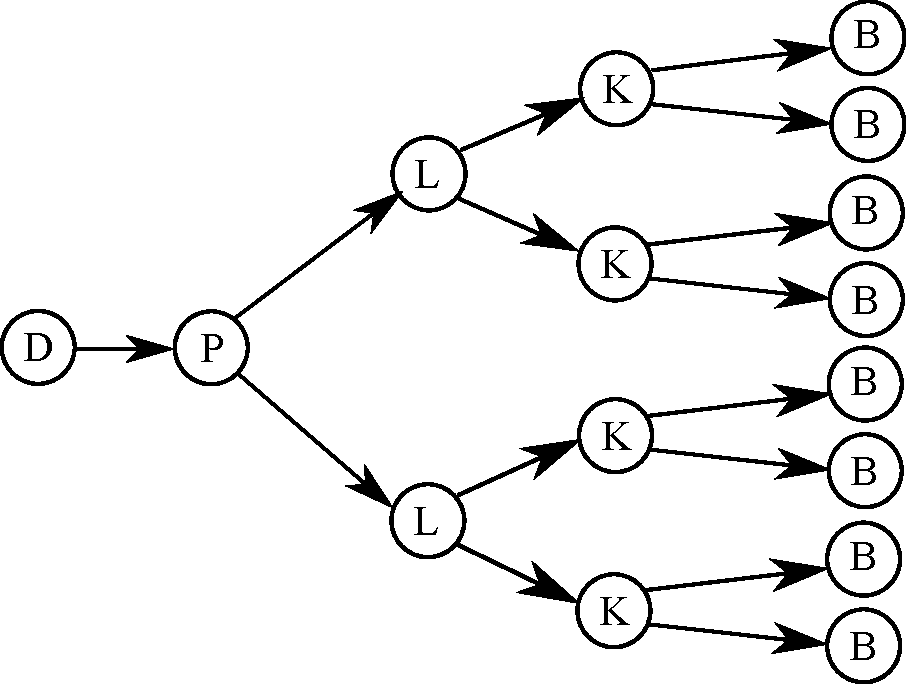
\includegraphics[width=10cm]{interessenter.pdf}
	\center\caption{Viser princippet bag, hvordan lampen overføres mellem de fem interessenter designer(D), producent(P), lampebutik(L), kunde(K) og bruger(B).}
    \label{fig:interessenter}
\end{figure}
% Sælgeren bliver også indirekte ramt, hvis mange kunder henvender sig fordi de gerne vil have en lampe returneret og byttet, så kræver det ressourcer fra lampebutikkers side. Derfor vil det også være til lampebutikkers fordel, at en kunde vil være i stand til at købe "den rigtige" lampe første gang eller en lampe, der er lidt dyrere fordi den giver den ønskede effekt.

\subsubsection{Designere}
Designere er interesseret i at deres design bliver solgt og er derfor sandsynligvis interesseret i et program, der kan hjælpe dem med at gøre deres design mere populært.

 
Vi har haft kontakt med to forskellige lampedesignere, danske Erik Mortensen, og svenske David Wahl fra IKEA. De sagde følgende:
\begin{center}
\textit{"I alle mine lamper er valg af lyskilde og placering sket på grundlag af test via prototyper. De fleste af mine lamper er prototyper"}.

\textit{"Jeg har i en del år arbejdet med lampedesign. og har derfor mest været optaget af armaturets/lampens skulpturelle udtryk, men da det jo er en lampe skal den selvfølgelig  også opfylde det belysningsmæssige."} Mailen kan ses i bilag \ref{sec:mailErik}.
\end{center}
og
\begin{center}
\textit{"Apart from hand sketching and physical prototypes, we use the 3D modeling application Solid Works in IKEA of Sweden. And for renderings we use either the built in renderer, or photo works, which is also part of solid works."} Mailen kan ses i bilag \ref{sec:mailDavid}.
\end{center}

Her er to eksempler på forskellige måder for designere, at visualisere en lampes lys på. Erik Mortensen benytter sig kun af prototyper, hvorudfra han kan se, hvordan lyset falder, hvorimod David Wahl, udover prototyper, også benytter sig af computerprogrammet Solid Works, til at visualisere lampens lys. 

\subsubsection{Producenter}
Producenten samarbejder med designeren om at udvikle lampen. Producentens rolle er at fremstille lampen på baggrund af designet. Når lamperne er produceret sendes de ud til lampebutikkerne. Producenten har en interesse i, at kunderne køber deres produkter i lampebutikkerne, da der er mulighed for, at dette vil medføre at lampebutikkerne bestiller flere af deres produkter hjem. En belysningskonsulent som vi har været i kontakt med, siger følgende om producenternes interesse i problemet: \textit{"Det er blevet en kompliceret proces at producere en lampe ift. EU lovgivning i dag så jeg har svært ved at se at producenterne vil koste endnu flere penge til produkter til privatmarkedet som måske kun køber en lampe til 3000 kr. som ofte kun interesserer sig for den laveste pris og ikke den bedste service og rådgivning. Så producenters incitament til ligge investeringer hos privatkunder er meget begrænset."} Mailen kan ses i bilag \ref{sec:mailbelysning}. Lampekonsulenten mener altså at producenterne ikke vil smide en masse penge ind i privatmarkedet, da det ikke gavner dem økonomisk. 

\subsubsection{Lampebutikker}
Lampebutikken er interesseret i at sælge flest mulige lamper, da dette giver større indkomst for butikken. Derudover er butikken også interesseret i, at kunden køber den 'rigtige' lampe første gang, da butikken på denne måde undgår utilfredse kunder, som vil returnere lamperne.

\subsubsection{Kunder}
Kunden er interesseret i at visualisere hvordan lys udbreder sig fra en lampe, da dette vil hjælpe kunden med at afgøre hvordan lampen passer ind i en kontekst, og kunden kan derfor undgå fejlkøb. Dette er kunden interesseret i, da det i sidste ende vil gavne brugeren af lampen, hvis kunden er i stand til at købe en lampe som passer ind i konteksten.

\subsubsection{Brugere}
Det er brugerne der i sidste ende benytter sig af lamperne i deres hjem eller på deres arbejde. Dette gør brugerne til den gruppe af interessenter, som påvirkes direkte af problemet, da de må leve med konsekvenserne, som belysningen fra en lampe kan medføre[HENVIS TIL AFSNIT OM KONSEKVENSER VED LYS]. Dette kan bl.a.\ være kontorarbejdere i en virksomhed, som påvirkes, hvis lamperne på deres kontor ikke passer sammen med indretningen. Et andet eksempel på brugere, er hjemme i privaten, hvor der kan være mange forskellige typer lamper, som skal passe ind i hjemmet. Hvis en person i hjemmet køber en lampe, som har en belysning, der ikke passer ind i hjemmet pga.\ manglende visualisering ved købet, så vil dette påvirke brugerne i hjemmet. 

\subsubsection{Økonomiske konsekvenser}
Når en kunde har valgt at investere i en lampe, uden at have haft muligheden for at visualisere lampens lys på en ordentlig måde på forhånd, kan det have økonomiske konsekvenser for én eller flere interessenter. Kunden, der køber en lampe, som de er utilfredse med, kan i de fleste situationer ikke få byttet produktet, da den originale emballage er brudt, og ledningen er pillet ved. Dette kan føre til en utilfreds kunde, som muligvis skal ud og investere i en ny lampe, og en lampebutik, med en potentiel utilfreds kunde, da de ikke har sørget for, at kunden kunne visualisere præcis hvordan lampen og dens lys ville se ud. Lampebutikken kan derfor opleve et mindsket salg af en hvis lampe, hvilket kan resultere i et mindsket antal af lamper, som de køber hjem fra producenten. Dette kan endvidere medføre et mindsket antal af producerede lamper, og som i sidste ende kan ende med at designeren også får færre penge.

\subsubsection{Målgruppen}
Som beskrevet i forrige afsnit, er det både designere, producenter, butikker, kunder og brugere, der påvirkes af problemet. Det er nu relevant at afgøre hvem problemløsningen retter sig mod, da dette danner grundlag for, hvordan løsningen skal udvikles og hvem der kan indrages i løsningen og udarbejdelsen af løsningsforslaget.

Som illustreret på figur \ref(fig:interessenter) er det lampebutikkerne, som har den direkte kontakt til kunderne og via kunderne en forbindelse til brugerne. Designere er fravalgt, da vi ud fra mails fra Wahl og Mortensen kan uddrage, at de allerede har værktøjer til at visualisere lys fra lamper, og som der ses på skitsen har designeren ikke nogle direkte kontakt til kunden eller brugeren. Man kunne forestille sig, at problemet kunne løses allerede fra producentens side af. Ud fra korrespondance med en belysningskonsulent i en lampebutik er dette dog blevet afvist. Vi er blevet informeret om, at producenterne ikke er interesseret i at bruge ressourcer på at løse problemet, da det ikke gavner producenterne direkte. Derudover er det ikke producentens opgave at vejlede kunder til det bedste køb af lamper, dette er derimod lampebutikken opgave.

Hvis man retter problemløsningen mod lampebutikker, og laver en løsning der gør det muligt for kunder at visualisere lamperne bedre, er det sandsynligt at kunderne vil være mere tilfredse med deres lamper, da de har mulighed for at se lampens belysning inden købet. For lampebutikker kan dette betyde, at kunden ikke returnerer lige så mange lamper, og dette vil bidrage til øget kundetilfredshed, som i sidste ende gavner både lampebutikker og kunderne. Hvis kunden er i stand til at købe en lampe som passer ind i den korrekte kontekst vil dette tilfredsstille brugeren. 


\subsubsection*{Opsummering}
I afsnittet er der blevet argumenteret for, at det er lampebutikker og brugere der bliver ramt af problemet, men at det vil være mest fordelagtigt at rette løsningen mod lampebutikker, da dette også løser problemet for brugerne.

Dette afsnit er relevant i forhold til den senere problemformulering, da der er blevet argumenteret for hvem det er, som har problemet, samt hvilken målgruppe det senere produkt skal udvikles til.

\clearpage
\subsection{Problemets placering}
I dette afsnit undersøges det hvor og i hvilke situationer problemet opstår for målgruppen. Da problemet tager udgangspunkt i købet af lampen, beskrives der, hvordan købssituationen er ved hhv. handel i fysiske butikker (Detail-handel) og handel i internetbaserede butikker (e-handel). Ud fra disse undersøgelser sammenlignes detail-handel og e-handel, for at afgøre hvor problemet er størst, og derudfra vælge den hvilken af type handel, som denne rapport ønsker at løse problemet indenfor.

\subsubsection{Detailhandel}
En fysisk butik er et sted hvor kunderne selv skal komme hen, når de vil købe eller kigge på butikkens varer. En fysisk butik har et ansat personale, som tager sig af butikkens kunder, og kan besvare deres mulige spørgsmål til butikkens varer. En fysisk butik er grundet det ansatte personale mm. dyr i omkostning, men kunderne foretrækker de fysiske butikker, da man kan se den virkelige varere selv og få direkte assistance om varen gennem en medarbejder\cite{fysisk_kontra_online}. Det kræver dog stadig at kunden selv skal ud til butikken, og være sikker på dens åbningstider og varelager.

I vores kontekst snakker vi om en hvilken som helst fysisk butik, der har med lampesalg at gøre. Den lampeinteresserede kunde, kommer ud i butikken, og leder fx efter en ny væglampe til stuen. Problemet heri kan opstå, ved at der er adskillige forskellige lamper at vælge imellem, men ikke alle lamperne er tilsluttet, så man kan se hvordan lyset falder. 
\newline Ved køb af lamper i den fysiske butik, er det ikke altid, at de lamper, som stilles frem til udstilling giver et realistisk billede af, hvordan lyset udbreder sig, da der ofte er mange lamper og lyskilder tæt samlet. Et andet problem er returretten. Returretten er ikke obligatorisk at have for fysiske butikker, så det er altså op til den enkelte butik/butikskæde, om de vælger at gøre det muligt at returnere en vare, selvom den er uåbnet og stadig i original emballage\cite{fortrydelsesret}. Hvis kunden beslutter sig for en lampe, som ikke er tilsluttet, men regner med at den vil se godt ud på væggen i stuen, hvorefter det så viser sig, at lyset falder helt forkert og er alt for skarpt og blændende er det for sent, da lampen er pakket ud, og ledningen er blevet pillet ved. Lampen kan altså ikke byttes, og er ikke optimal i forhold til kundens stue. Der er mange butikker og butikskæder, som vælger at gøre det muligt for kunden at bytte en vare, hvis den stadig er i original emballage og med kvittering \cite{ikea_returret}, men det er ikke noget, som butikker er tvunget til at gøre, og med en lampe som eksempel, kan man ikke tage den med hjem og ’afprøve’ den, uden at annullere sin returret, da den bliver pakket ud og ledningerne bliver pillet ved.


\subsubsection{E-handel}
\label{sec:ehandel}
E-handel er elektronisk handel via internettet\cite{ddo_ehandel}. På internettet kan sælgere inden for e-handel have såkaldte e-butikker, hvor kunder kan købe varer\cite{ddo_ebutik}. E-butikker er ofte udformet således at kunden kan se billeder og informationer omkring sælgerens varer og derudfra kan kunden vælge at lægge varerne i en virtuel indkøbskurv, hvor kunden til sidst indtaster de nødvendige oplysninger for at købe og modtage varerne.


Blandt de mange forskellige varer, der sælges via e-butikker, er det her relevant at tale om e-handel med lamper. Nedenstående figur \ref{fig:e_handel_med_lamper} illustrerer princippet bag en lampesælgers salg af lampe til en kunde via en e-butik.
\begin{figure}[H]
	\centering
	\def\svgwidth{\columnwidth}
	\input{./graphics/e_handel_med_lampe.pdf_tex}
	\caption{Princippet bag handel af en lampe via en e-butik.}
    \label{fig:e_handel_med_lamper}
\end{figure}

På figur \ref{fig:e_handel_med_lamper} er det vist hvordan e-handlen starter med at kunden får et udvalg af lamper fra e-butikken. Kunden sender så en bestilling, som via e-butikken sendes videre til lampesælgeren, og til sidst sendes lampen til kunden. Dog ender handlen ikke nødvendigvis her, da kunden kan sende lampen retur såfremt at gældende lovgivning og købsbetingelser muliggører dette. For at undersøge lovgivningen nærmere kan man tage udgangspunkt i den danske lov om forbrugeraftaler\cite{retsinformationen}.

I lovens kapitel 1, § 1, stk. 2, nr. 1, fremgår der at lovens bestemmelser for fortrydelsesret gælder for aftaler, som er indgået ved fjernsalg. For en  fjernsalgsaftale gælder der, at aftalen om varer, er indgået gennem fjernkommunikation, hvor den erhvervsdrivende og forbrugeren ikke mødes fysisk (jf. kap. 1, § 3, nr. 1).

Ser man nu på loven i forbindelse med e-handel, foregår fjernkommunikationen gennem internettet via e-butikken, hvor fjernsalgsaftalen udføres i form af brugerens bestilling af f.eks. en lampe. Dette gør at fortrydelsesretten gælder ved e-handel.

Fortrydelsesretten er en forbrugers mulighed for at melde sig ud af en aftale, herunder køb af lamper ved e-handel. Hvis en en forbruger eksempelvis køber en lampe via en e-butik, har forbrugeren mulighed for at fortryde købet inden 14 dage ved at meddele dette til den erhvervsdrievende (jf. kap. 4, § 19). Herefter har forbrugeren 14 dage til at returnere varen (jf. kap. 4, § 24). Hvis varens værdi er forringet som følge af forbrugerens unødvendige håndtering af varen for at inspicere denne, så hæfter forbrugeren for værdiforringelsen (jf. kap. 4, § 24, stk. 5). Dvs. at hvis en bruger installerer og bruger lampen, hvor der f.eks. tilpasses ledninger, så kan lampens værdi forringes og forbrugeren skal hæfte for dette. 

\subsubsection{Sammenligning af detail- og e-handel}
Ud fra ovenstående redegørelse af de to typer for handel, analyseres disse nu med henblik på at finde ligheder og forskelle, hvoraf det kan afgøres i hvilken af de to typer af handel, at problemet er størst. 

Da det initierende problem er at forbrugeren ikke kan visualisere lampen uden at købe den, er det derfor relevant at se på i hvor høj grad dette er tilfældet ved de to typer handler.

Fordelen ved detail-handel, er at forbrugeren ofte kan se lampen i butikken, og ud fra dette, vurdere hvilken lampe der opfylder de behov som forbrugeren har. Dog er problemet stadigvæk at forbrugeren ikke ser lampen i den rette kontekst, dvs. i sit eget hjem. Dette kan gøre at forbrugeren får et godt indtryk af lampen i den kontekst, som butikken præsenterer den i, men at den ikke passer ind i den kontekst, som forbrugeren køber lampen til.

Ved e-handel har forbrugeren ikke muligheden for at se en fysisk udgave af lampen, men ofte kun billeder. Dette gør at forbrugeren alene kan tage valg ud fra de billeder og informationer, som e-butikken præsenterer. Problemet er så, at billederne til dels ikke er interaktive, dvs. brugeren ikke kan se lampen fra flere vinkler end dem som billederne er taget i, samt at billederne ikke er taget af lampen i den kontekst, som forbrugeren ønsker at købe lampen til. 

Med hensyn til konteksten er fordelen ved e-handel, at forbrugeren kan sidde derhjemme, i den kontekst, hvor lampen skal indgå, og sammenligne med de informationer, der er tilgængelige på e-butikken. I modsætning til dette er detail-butikker, hvor forbrugeren står i butikken, og måske har problemer med at huske eller blot forestille sig alle detaljerne ved den kontekst, som lampen skal indgå i.

Ud fra denne sammenligning, er der på den ene side detail-handel, hvor det er svært at visualisere konteksten, men hvor man kan se lampen. På den anden side er e-handel, hvor man kan sidde derhjemme i konteksten, men har svært ved at visualisere lampen. 

For at afgøre hvilken type handel denne rapport vil fokusere på, skal der derfor svares på om det er mangel på visualisering af lampen i kontekst ved detail-handel eller mangel på visualisering af lampen ved (e-handel), som er det største problem.

Da forbrugeren omgås og ser den kontekst, som lampen skal indgå i f.eks. et kontor, køkken og bad, så må man kunne antage at forbrugeren har en forestilling om, hvordan denne kontekst ser ud selvom forbrugeren ikke står i den når der handles i en fysisk butik. Derfor er dette ikke et lige så stort problem, som hvis forbrugeren ikke kan visualisere lampen når der handles via e-handel. Derfor vil fokuset i denne rapport være at forbedre forbrugerens evne til at visualisere lamper under e-handel.

\subsubsection{Opsummering}
Trods at problemet opstår hos forbrugeren, altså at de har problemer med at visualisere den givne lampe fra alle vinkler og i det rette miljø, er der ingen måde, hvorpå forbrugeren selv kan løse dette problem på en let og effektiv måde. Vi vil derfor fokusere på hvordan  problemet kan blive løst, allerede før varen når ud til forbrugeren. Derfor er vi nødt til at fokusere på sælgeren (e-handelsbutikker), når det kommer til løsningen af viasuleringsproblemet. Her kunne det tænkes, at der kunne udarbejdes et værktøj, der ville forbedre og optimere forbrugerens visualisering af den givne lampe.






\clearpage
% \subsection{Teknologianalyse}
% \label{sec:teknologianalyse}
% Vi ser en tydelig mulighed for at assistere forbrugere med at træffe et valg, når det kommer til køb af varer på nettet, bestemmelse af optimale lysforhold i hjemmet og visualisering af et tilkøbt element i forbrugernes dagligdag/hjem. Dette vil sandsynligvis kunne løses ved hjælp af bedre købsvejledning eller værktøjer til at assistere forbrugeren i en købssituation hvor en prøve ikke kan stilles til rådighed eller at returnere varen er umuligt eller for omfattende en process.

% % // redegørelse
% Blot at vælge en lampe fra et katalog er problematisk, hvis der ikke er billeder af lampen som
% \begin{enumerate}
%     \item Fremviser lampen som møbel, rent visuelt, det fysiske design og 
%     \item Viser hvordan lys kastes af lampen. En god løsning vil være at have en fysisk model placeret i en kontekst hvor man kan komme og se lampen og se lyset i sammenspil med anden indretning, således som f.eks. Ikea gør.
% \end{enumerate}

% Man vil også kunne skabe billige prototyper af lamper vha. 3D printer teknikker. Disse ville eventuelt være mulige at tage med hjem for at teste hvordan en lampe passer ind i det rum den egentligt er købt til, men fordi plastik vejer mindre end metal, glas og andre tunge materialer som lamper kan være produceret af, kunne man forestille sig ophængsmetoder der ikke nødvendiggør at bore huller i vægge, før man har set om lampen passer ind i rummet.

% En tredje metode kunne være at konstruere en 3D model af lampen og køre en simulation af, hvordan den kaster lys. Dette koncept vil også kunne udvides til, at en forbruger kan modellere deres eget hjem og placere lampen i den model af deres hjem som de opstiller. Eller det kan anvendes af lampebutikker som et værktøj til at vejlede forbrugeren til at påtage det rigtige køb.

% Indledning over



\subsection{Afgrænsning af løsningsfelt}
For at visualisere hvilken afgrænsning af løsningsfeltet, der nu er foretaget, har vi, ud fra ovenstående problemanalyse, fremstillet figur \ref{fig:p1_skitser}, der viser løsningsfeltet for det initierende problem. Figuren viser på den lodrette akse hvem der styrer visualiseringen af lamper, og den vandrette akse viser, hvor lamperne visualiseres. I feltet er fire løsningsmuligheder vist.

\begin{figure}[H]
  
  \centering
  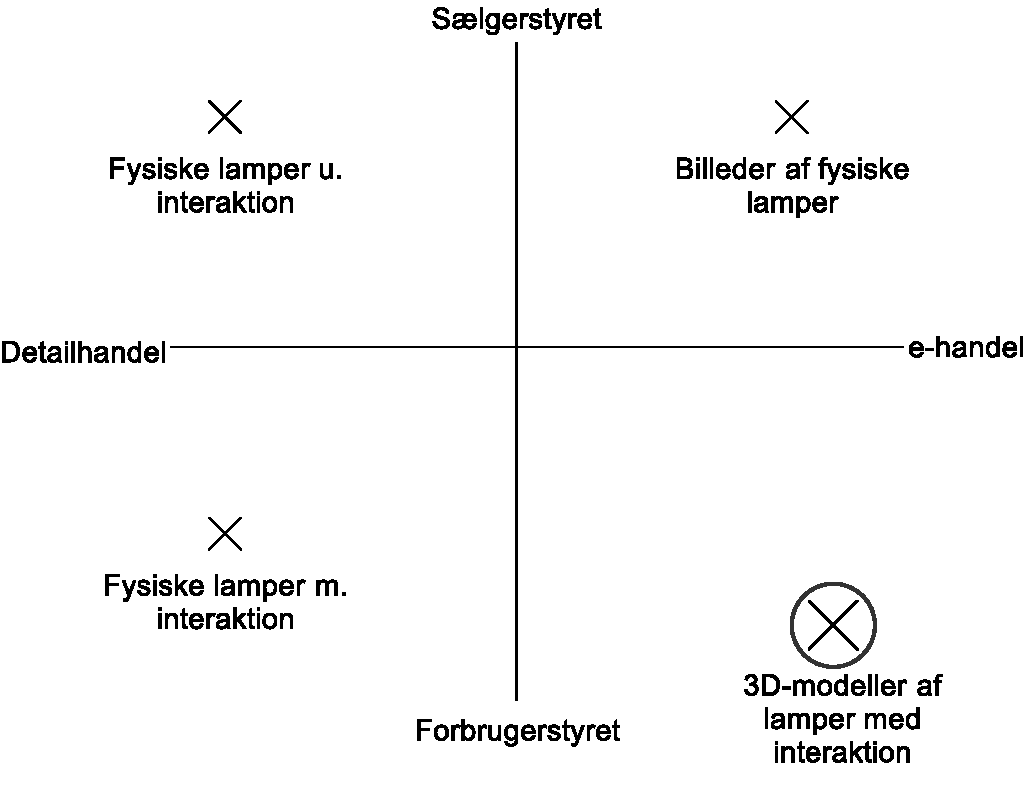
\includegraphics[width=10cm]{p1_skitser}
  \caption{Illustrerer lønningsfeltet til initierende problem, hvor det afgrænsede løsningsfelt er markeret med en cirkel.}
  \label{fig:p1_skitser}
\end{figure}

Herunder er de fire løsningsmuligheder, vist på figur \ref{fig:p1_skitser}, beskrevet:
\begin{enumerate}
  \item fysiske lamper uden interaktion, som er de lamper lampebutikker udstiller i fysiske butikker, men som forbrugeren ikke har mulighed for interaktion med, det vil sige at dette ofte er lamper som er slukket.

  \item fysiske lamper med interaktion, som er de lamper lampebutikker udstiller i fysiske butikker og som brugeren bl.a.\ kan slukke og tænde for, altså have interaktion med.

  \item billeder af fysiske lamper på e-butikker. Her har kunden mulighed for at se et billede af lampen, men kun fra de vinkler og i den kontekst som lampebutikken har valgt.

  \item 3D-modeller af fysiske lamper m.\ interaktion på e-bukker. Her har kunden mulighed for at se et 3D billede af lampen samt rotere lampen, og herved se hvordan lampens belysning er fra de ønskede vinkler, og ikke kun i den kontekst som lampebutikken vælger det. 
\end{enumerate}

Figuren viser nu at det er løsningsmulighed 4, som der afgrænset til i løbet af problemanalysen, og vi dermed har fravalgt løsningsmulighed 1-3 på baggrund af problemanalysen. Dette gør at der nu kan opstilles en endelig problemformulering, som ligger op til en løsningsmulighed 4.
\clearpage
